\section{Security-Enhanced Closures}\label{concepts:secure_closures}

Section \ref{concepts:closures} states that the closure is the execution
primitive of the TEM, and illustrates the structure of a closure. It follows
that the TEM's mission is to provide trusted execution for closures.
According to section \ref{concepts:guarantees}, this is equivalent to
guaranteeing integrity and confidentiality.

Section \ref{concepts:information_classes} classifies the information
inside a closure as \textit{private}, \textit{shared}, or \textit{open},
according to the guarantees needed. A \textbf{Security-Enhanced Closure (SEClosure)}
is a closure with all the information classified as described above.

Before they can be executed by the TEM, SEClosures must be compiled and encoded in a format that is easy to process, so that the logic to be implemented inside the TEM is minimized. The rest of this work uses the term \textbf{SECpack} to refer to compiled and encoded SEClosures.

SECpacks are suitable to be executed by the TEM, but the information inside
them is unprotected. Section \ref{concepts:secpack_binding} describes a
process that uses a TEM's Public Encryption Key (PubEK) to produce a
\textbf{bound SECpack}. The bound SECpack contains the same information as the
original SECpack, but it enforces the confidentiality and integrity of the
information it contains. Thefore, Yu can safely give Mii a SECpack that was
bound to Mii's TEM. The term \textit{bound} is justified by the fact that a
bound SECpack can only be used by the TEM whose PubEK was used to produce the
bound SECpack.

\subsection{Security Guarantee Classes}\label{concepts:information_classes}

Section \ref{concepts:guarantees} shows that trusted execution is equivalent
to providing integrity and confidentiality guarantees. However, both guarantees
are not needed by all the information expressing a computation. Therefore it
makes sense to classify the information, according to the guarantees needed:
\begin {itemize}
  \item \textbf{private}: this is information that requires the confidentiality
  guarantee. Examples of secret information are Yu's social security number, or
  one of her private encryption keys.
  \item \textbf{shared}: this is information that only requires an integrity
  guarantee. In the back account example in section \ref{concepts:closures}, if 
  the code for \texttt{withdraw} can be changed to the code for
  \texttt{deposit}, that would have dramatic consequences on the bank.
  \item \textbf{open}: this information is not covered by any guarantee. This
  has to be information that Mii supplies to the computation. As described in section
  \ref{concepts:use_model}, Mii is the TEM's owner, and therefore he is the only
  one who would trust the platform automatically, without requiring any proof
  of integrity or confidentiality.
\end{itemize}

Private information must automatically receive an integrity guarantee, in order
to ensure no secret is leaked. For example, secrets are usually encryption or
signing keys. If Mii can replace one of Yu's key with his own, Yu's key will
still be confidential, but Mii can access any information encrypted by Yu's key.

Section \ref{concepts:guarantees} proves that all the executable code in a
closure requires an integrity guarantee. It follows that for trusted execution,
all the executable code in a SEClosure is either private or shared.

For reasons of simplicity, it seems appealing to remove the \textit{shared}
class of information, and specify that all the information originating from Yu
is private. However, if all the executable code is made private, then it is
impossible for Yu to prove Mii anything about the nature of the computation
expressed in the closure. The shared class is motivated by my conviction that
known information should not be encrypted, and by applications where Mii must
verify that the closure expresses a certain computation.

The next section describes a method for implementing the security guarantee
classes presented here, thus demonstrating that the idea is practical.

\subsection{Implementing the Security Guarantee
Classes}\label{concepts:secpack_binding}

The TEM's use model (section \ref{concepts:use_model}) states that the
information describing Yu's computation will pass through at least one
intermediary (Mii) before reaching the TEM. Therefore, it is reasonable to
assume that the information can be altered arbitrarily in the passage from Yu
to Mii's TEM.

Fortunately, Yu can be assumed to know the TEM's Public Endorsement Key
(PubEK), and she can use it to communicate secrets securely to the TEM,
according to section \ref{concepts:trust_chain}. The following process,
illustrated in figure \ref{fig:secpack_binding}, uses the Public Endorsement Key to
convert a SECpack into a form that provides the appropriate guarantees (section
\ref{concepts:information_classes}) for the information inside the SECpack,
despite the fact that the information has to pass through Mii's hands.

\begin{figure}[hbtp]
	\center{
		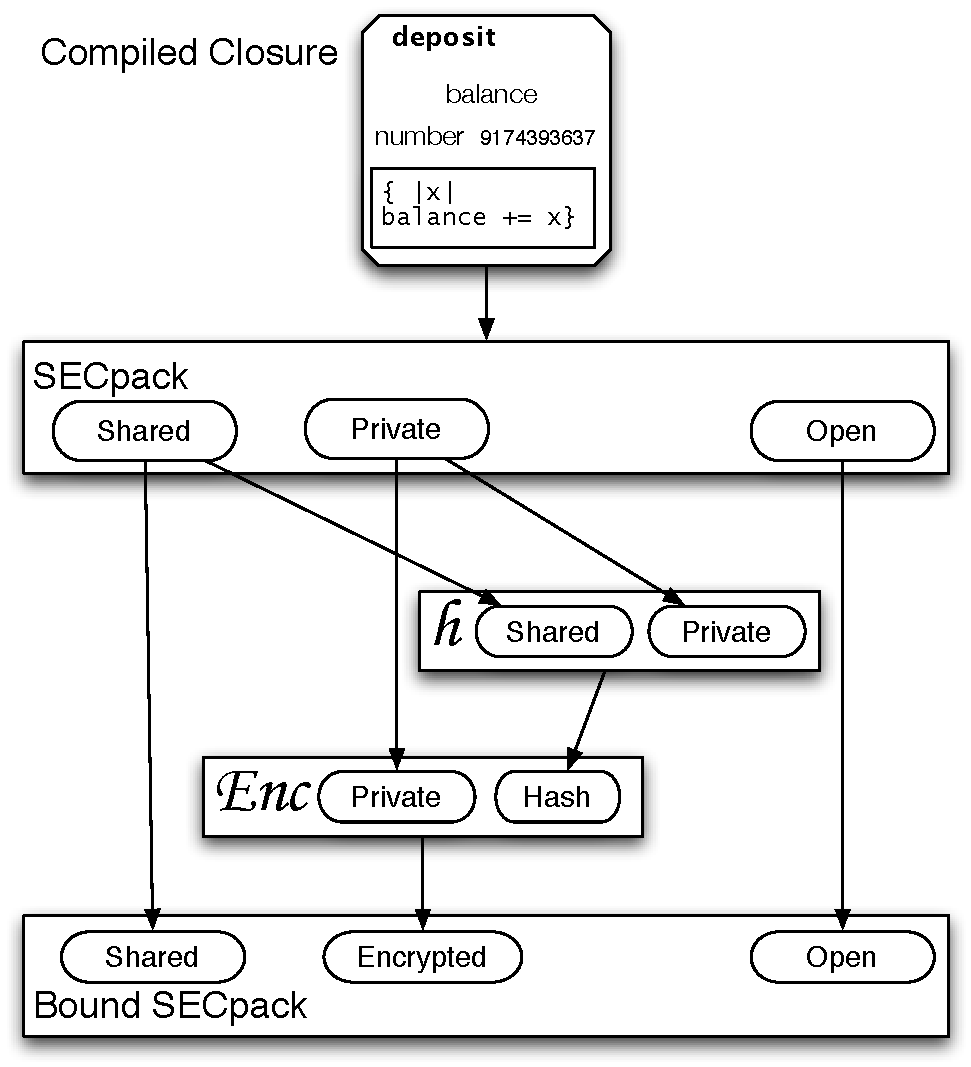
\includegraphics{omnifigs/secpack_binding}
	}
	\caption{Securing the Information in a Closure}
	\label{fig:secpack_binding}
\end{figure}


\begin{enumerate}
  \item Let $\mathcal P$ be the private information, $\mathcal S$ be the shared
  information, and $\mathcal O$ be the open information.
  \item Use a cryptographic hashing function $h$ (such as SHA1
  \cite{eastlake2001rus} or MD5 \cite{rivest1992rmm}) to compute a message
  digest of the private and the shared information. $$\mathcal H = h(\mathcal P
  || \mathcal S)$$ Note: $||$ denotes concatenation.
  \item Use the TEM's Public Endorsement Key to encrypt the private information
  together with the message digest. $$\mathcal E =
  {\mbox{\Large \textit{Enc}}}_\textrm{PubEK}\Big(\mathcal P || \mathcal
  H\Big)$$
  \item The secured closure consists of the encryption result $\mathcal E$,
  together with the shared information $\mathcal S$, and the open information
  $\mathcal O$. $$\textrm{Secured Closure} = (\mathcal S || \mathcal E ||
  \mathcal O)$$
\end{enumerate}

Yu will follow the process above to secure her closure before transmitting it
to Mii. When Mii's TEM will receive the closure, it will use its Private
Endorsement Key (PrivEK) to decrypt $\mathcal E$ and obtain $\mathcal P$ and
$\mathcal H$. In order to guarantee integrity and privacy, the TEM will refuse
the input if $\mathcal H$ doesn't match the hash of $\mathcal P || \mathcal S$.
This is sufficient to provide the security guarantees for private and shared
data, as proven by the following:

\begin{theorem*}
The scheme described above guarantees the confidentiality of the
private information $\mathcal P$ and the integrity of the shared information $\mathcal S$ and
the private information $\mathcal P$.
\end{theorem*}
\begin {proof}
By strong induction over $N_E$, the number of execution attempts of the secured
closure on Mii's TEM. Note that an execution attempt can fail, if Mii attempts
to change $\mathcal P$ and/or $\mathcal S$ in the closure (the fact follows
immediately from this theorem).

\textbf{Base case.} the guarantees are provided on the secured closure's first
execution attempt.

$\mathcal P$ cannot be directly derived from $\mathcal E$, assuming the
encryption algorithm associated with PubEK is resistant to Mii's
attacks\footnote{This is believed to be true, at least
for RSA \cite{rivest1978mod} and ECC \cite{koblitz1987ecc}.}, and that $h$ is
inverse-resistant\footnote{It is impossible to compute $\mathcal P || \mathcal
S$ from $H$. This is true for any good cryptographic hash function, and it is
believed to be true for SHA1 \cite{eastlake2001rus} and MD5
\cite{rivest1992rmm}.}. As a special case, note that $\mathcal P$ will never be
empty, because the trusted execution assumption implies the existence of
confidential information, as proven in section \ref{concepts:guarantees}.

Assuiming $\mathcal P$'s confidentiality (proven above), it follows that, in
order for Mii to mutate $\mathcal S$ to $\mathcal S'$, Mii must break $h$ as
well as ${\mbox{\Large \textit{Enc}}}_\textrm{PubEK}$ in order to produce
the correct values of $\mathcal H'$ and $\mathcal E'$ without knowing
$\mathcal P$.

The process is resistant to modifications of $\mathcal P$
as well, as long as the entire value of $\mathcal P$ is not replaced. Assume
the mutation transforms $\mathcal P = (P_\alpha || P_0 || P_\Omega)$ into
$\mathcal P' = (P_\alpha || P_1 || P_\Omega)$. The argument in the previous
paragraph can be used to show that Mii must break $h$ and ${\mbox{\Large
\textit{Enc}}}_\textrm{PubEK}$, since he does not know $P_\Omega$ and/or
$P_\alpha$ (at most one of them may be empty).

Therefore, Mii cannot determine his TEM to execute the secured closure with
modifications to $\mathcal P$ or $\mathcal S$ without replacing $\mathcal P$
completely. But once $\mathcal P$ is replaced with a value known by Mii, the
closure does not contain any of Yu's secrets. Therefore, the notion of trusted
computation isn't applicable to the resulting closure -- the computation in it
can be specified by Mii alone, and executed on any platform.

\textbf{Induction step.} assuming the guarantees are provided on the secured
closure's first $N_E$ execution attempts, I will prove that the guarantees will
be provided on the $(N_E + 1)^\textrm{th}$ attempt.

$\mathcal P$'s integrity is guaranteed for attempts $1 \ldots N_E$, so the TEM
cannot be used to execute closures containing arbitrary mutations of $\mathcal
P$. Therefore, no information about $\mathcal P$ is leaked in the first $1
\ldots N_E$ attempts. Hence, recovering $\mathcal P$ on the $(N_E +
1)^\textrm{th}$ attempt is just as difficult as recovering it directly from $\mathcal E$.
Therefore, the assumptions of the base case still hold, and the same argument
can be used for the induction step.
\end{proof}
